%%%%%%%% ICML 2021 EXAMPLE LATEX SUBMISSION FILE %%%%%%%%%%%%%%%%%

\documentclass{article}
\usepackage{float}
\usepackage{microtype}
\bibliographystyle{icml2021}
\usepackage{graphicx}
\usepackage{subfigure}
\usepackage{booktabs}
\usepackage{float}
\usepackage{gensymb}
\usepackage{amsmath}
\usepackage{amssymb}
\usepackage{tikz}

\usepackage{url}
\def\UrlBreaks{\do\/\do-}
\usepackage{breakurl}
\usepackage[breaklinks]{hyperref}
\usepackage{hyperref}

\newcommand{\theHalgorithm}{\arabic{algorithm}}
\newcommand{\TODO}[1]{\textcolor{blue}{#1}}

\usepackage[accepted]{icml2021}

\icmltitlerunning{Hyperparameter Tuning using Evolutionary Algorithms}

\begin{document}

\twocolumn[
\icmltitle{Hyperparameter Tuning using Evolutionary Algorithms}
\icmlsetsymbol{equal}{*}
\begin{icmlauthorlist}
    \icmlauthor{T. Blom (sXXXXXXXX)}{LIACS}
    \icmlauthor{J. Hamelink (s2233827)}{LIACS}
    \icmlauthor{L. Peeters (sXXXXXXX)}{LIACS}
    \icmlauthor{S. Sharma (sXXXXXXX)}{LIACS}
\end{icmlauthorlist}
\icmlaffiliation{LIACS}{LIACS, Leiden University, Leiden, Netherlands}
\icmlcorrespondingauthor{Mike Preuss}{LIACS}
\icmlkeywords{Hyperparameter Tuning, Evolutionary Algorithms, Reinforcement Learning}

\vskip 0.3in
]

\printAffiliationsAndNotice{}

% -------------------------------------------------------------------
% -------------------------------------------------------------------
\section{Introduction}
\label{sec:intro}
Hyperparameter tuning is an active research topic in machine learning that can have a significant impact on the performance of models. 
The process of manually fine-tuning hyperparameters can be time-consuming. 
In this study, we propose the use of a genetic algorithm as a means to optimize the hyperparameters of an Advantage Actor-Critic (A2C) agent. 
This includes the hyperparameters of the neural network the agent uses such as the number of layers, the number of neurons per layer, the activation functions employed, and the learning rate. Furthermore, hyperparameters of the A2C agent such as the discount factor, Entropy Regularization, and baseline subtraction. 
We aim to automate the exploration of various hyperparameter settings using a genetic algorithm, with the goal of finding an optimal combination. 
We use a bitstring representation to encode and manipulate the hyperparameter configuration. 
Each bit or set of bits within the string corresponds to a specific hyperparameter setting, allowing for easy manipulation by the genetic algorithm's evolutionary process. 
Similar to the process of natural selection and genetics, the genetic algorithm starts with an initial population of bitstrings and iteratively tries to improve them with the goal of finding an optimal configuration of hyperparameters. 
To evaluate the performance and effectiveness of our Hyperparameter Optimization (HPO) algorithm for the A2C agent, we apply the agent on three of OpenAI's Gym environments: CartPole-v1, Acrobot-v1, and LunarLander-v2. 
These environments provide varying sizes of action and observation spaces, enabling a more generalized assessment of the HPO algorithm's performance.
In this study, we aim to investigate the impact of our genetic algorithm-based HPO approach on the performance and convergence speed of the A2C agent in various Gym environments. 

% -------------------------------------------------------------------
% -------------------------------------------------------------------
\section{Methodology}
\label{sec:meth}

\TODO{small intro for this section.}

% -------------------------------------------------------------------
\subsection{Actor-Critic}
\label{ssec:ac}

\TODO{
    We do A2C.
    Pseudo-code and equations.
    Explain methods: 2-headed neural network, entropy regularization, baseline subtraction, advantage estimation (calculating returns).
    Mention that these params will be tuned using EA.
}

We don't use this paper, but it's just to show that the citations work \cite{han2020actorcritic}.

% EXAMPLE ALGORITHM
\begin{algorithm}[htbp]
    \caption{Actor-Critic}
    \label{alg:trunk}
    \begin{algorithmic}[1]
        \STATE {\bfseries Input:} environment, $\pi_\theta$, $V_\phi$
        \STATE \texttt{$\pi_\theta$} $\gets$ random values
        \STATE \texttt{$V_\phi$} $\gets$ random values
        
        \WHILE {not converged}
            \STATE Under policy $\pi_\theta$,
            \STATE sample episode $s_0, a_0, r_1, \dots, s_{T-1}, a_{T-1}, r_T$
            \STATE \texttt{G} $\gets$ discounted returns using equation \ref{eq:disc-ret}
            \IF {baseline subtraction}
                \STATE \texttt{G} $\gets$ \texttt{G} - \texttt{V}
            \ELSE
                \STATE \texttt{G} $\gets$ \texttt{G}
            \ENDIF
            \STATE Update $\pi_\theta$ and $V_\phi$ using \texttt{G}
        \ENDWHILE
    \end{algorithmic}
\end{algorithm}

% EXAMPLE EQUATION
\begin{equation}
    \label{eq:disc-ret}
    G_t = \sum_{k=0}^{\infty} \gamma^k r_{t+k+1}
\end{equation}

% -------------------------------------------------------------------
\subsection{Evolutionary Algorithm}

\TODO{
    EA is a population-based search algorithm.
    Pseudo-code and equations.
    Explain methods: deterministic selection, elitism, 1-p crossover, uniform mutation.
    Do not mention the settings chosen for parameters such as $\mu, \lambda$ and mutation rate yet.
}

% EXAMPLE TABLE
\begin{table}[htbp]
    \centering
    \begin{tabular}
        {|c|c|}
        \toprule
        \textbf{Parameter} & \textbf{Value} \\
        \midrule
        population size & 6 \\
        $\mu$           & 3 \\
        $\lambda$       & 3 \\
        mutation rate   & 0.1 \\
        \bottomrule
    \end{tabular}
    \caption{Hyperparameters}
    \label{tab:hyper}
\end{table}

% -------------------------------------------------------------------
% -------------------------------------------------------------------
\section{Experiments}
\label{sec:exp}

\TODO{
    List environments: CartPole, Acrobot, LunarLander.
    Explain why these environments were chosen (discrete action space, no input that needs conv layers).
    List bitstring makeup: what values for what params.
    Don't mention results yet.
}

% -------------------------------------------------------------------
% -------------------------------------------------------------------
\section{Results}
\label{sec:res}

\TODO{
    For each of the subsections, small introduction of what is to be expected.
    Then graphs and tables.
    Then (not super in-depth) analysis of the results.
}

% -------------------------------------------------------------------
\subsection{CartPole}
\label{ssec:cp}

\TODO{Lorem ipsum.}

% EXAMPLE FIGURE
\begin{figure}[htbp]
    \centering
    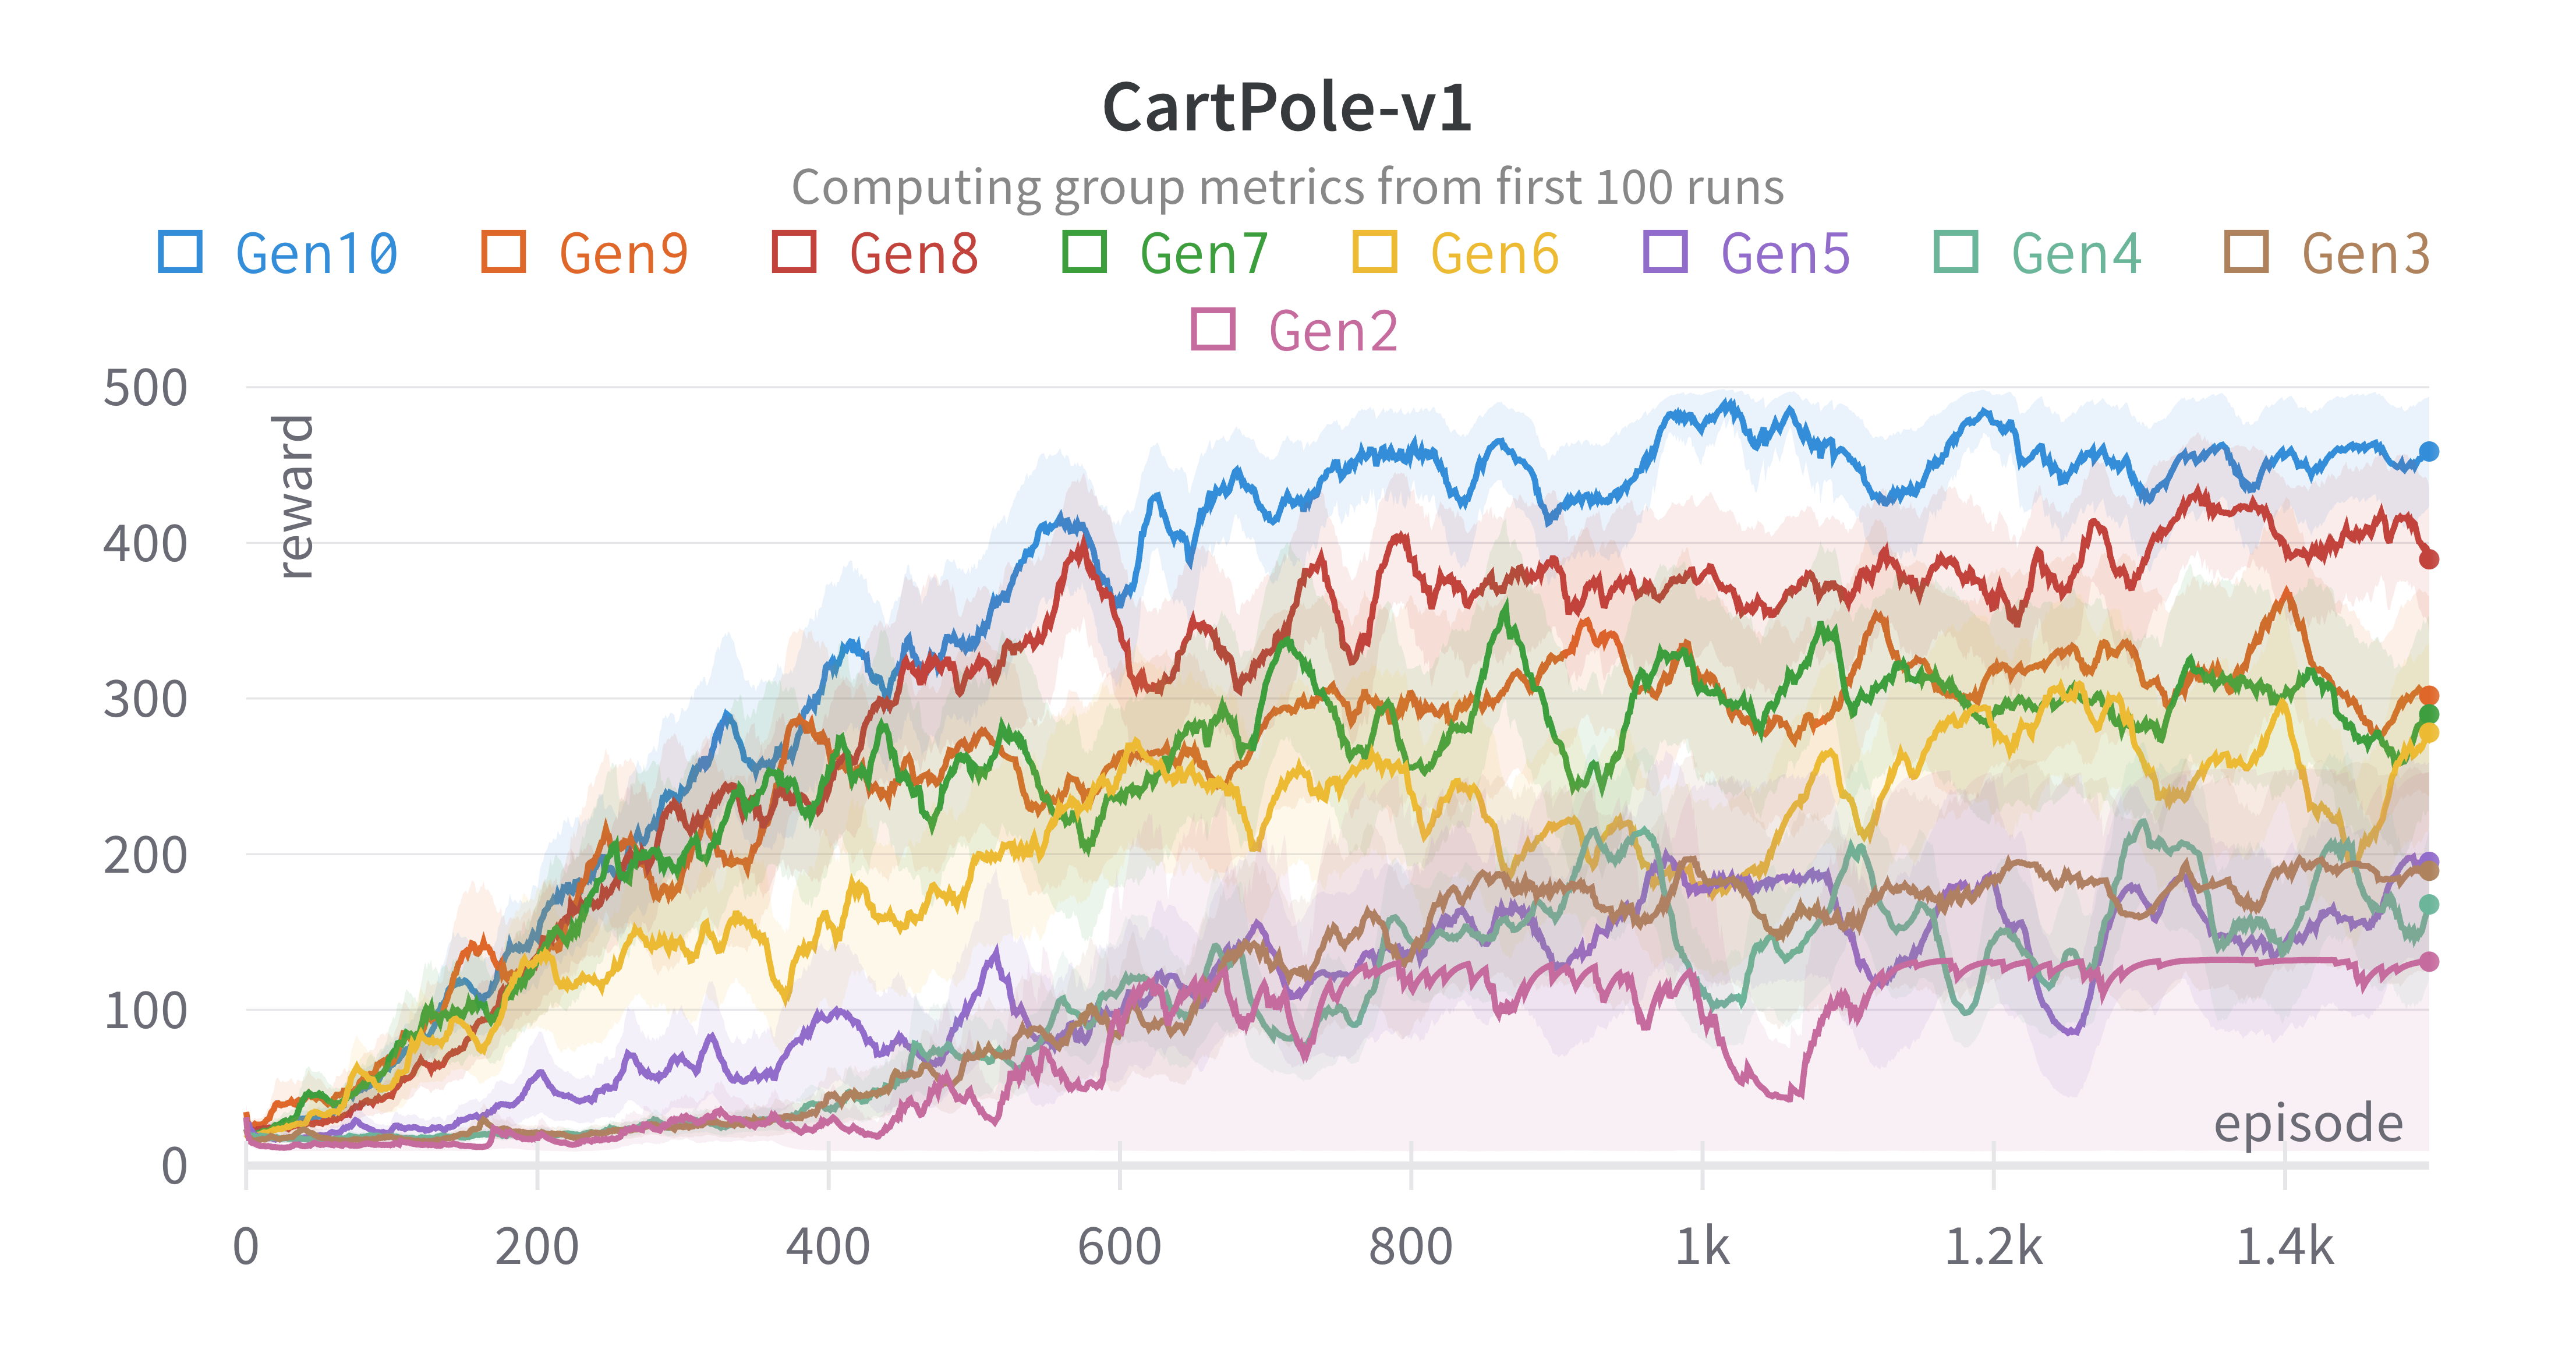
\includegraphics[width=0.9\linewidth]{figs/lc-cp.png}
    \caption{
        Be descriptive of what different colors/lines mean.
        A multi-line caption should be formatted as such.
        Try to not exceed 3 lines.
    }
    \label{fig:lc-cp}
\end{figure}

% -------------------------------------------------------------------
\subsection{Acrobot}
\label{ssec:ab}

\TODO{Lorem ipsum.}

% -------------------------------------------------------------------
\subsection{LunarLander}
\label{ssec:ll}

\TODO{Lorem ipsum.}

% -------------------------------------------------------------------
% -------------------------------------------------------------------
\section{Conclusion}
\label{sec:conc}

\TODO{
    What did we find, why are some architectures/params better than others for specific environment?
    Is EA a valid approach for this problem?
}

\section{Discussion}
\label{sec:disc}

\TODO{
    What could be improved?
    What could be done differently?
    What could be done next?
}

% -------------------------------------------------------------------
\bibliography{references}

\end{document}
